\documentclass[UTF8]{ctexart}
% \usepackage{amsfonts}
% \usepackage{amsmath}
% \usepackage{amssymb}
% \usepackage{amsthm}
% \usepackage{booktabs}
\usepackage{courier}
% \usepackage{float}
\usepackage{geometry}
\usepackage{graphicx}
\usepackage{hyperref}
% \usepackage{listings}
\geometry{left=2.54cm,right=2.54cm,top=2.18cm,bottom=3.18cm}

\begin{document}

\title{人脸表情识别报告}
\author{无46\ \ 黄秀峰\ \ 2014011193\\ 无46\ \ 严靖凯\ \ 2014011192\\ 无46\ \ 王启睿\ \ 2014011179}
\maketitle

\section{概述}

对于人脸表情识别问题,目前学术界已有了一定的研究,并且当前在该问题上有许多算法比赛,吸引着众多科研人员参与。比较典型的包括Kaggle的FERC,SSPNET的FERA,ACM的EmotiW,等等。这些比赛采用特定的数据集,有一些由实验室环境下采集的数据为主,另一些直接来自于实际图片或视频。

在本报告中,我们将首先说明我们选用的方法及原因,再对算法实现进行介绍,最后对判别结果进行分析,并指出可能的未来改进方向。

\section{选用方法的确定}

本节中,我们将介绍我们曾着重考虑过的两种方法以及最终选用方法的确定。其中一是采用WLD + HOG特征的传统模式识别方法,二是采用神经网络的特征提取识别方法。

\subsection{两种思路}

与目前大多数机器学习问题一样,对与人脸表情识别问题的处理方法,大体可分为传统模式识别和神经网络两类。其中,传统模式识别方式的代表性文章有
\cite{happy2015automatic,islam2016sention,wang2013feature,salmam2016facial}等,其中大多数采用SVM或决策树进行判决,神经网络方式的代表性文章有
\cite{BarsoumICMI2016,khorrami2015deep}等。传统方法往往训练和运行速度很快,部分方法甚至可以应用于实时视频流作为输入等场景,对于质量高(清晰、光照合适、正脸)的图片有很高的识别正确率;而神经网络方法对于很低的图片分辨率、不理想的光照、侧脸,或视频片段等情形的处理效果较好。

在我们本次实验任务中,我们面对两个主要挑战:一是需要对自采数据集进行判决,其中的图片与实验室中标准数据有很大区别;二是本次提供的训练图片数很少,只有521张。前者促使我们考虑神经网络的方法,但后者使得神经网络的训练条件不足。相比之下,传统方法在小数据样本情形下通常有更好的效果。

\subsection{神经网络的尝试}
根据我们所调研的文献,文章\cite{BarsoumICMI2016}提供的FER+数据集中有较多数据,因此我们选择在FER+数据集上复现文\cite{BarsoumICMI2016}的效果。

\begin{figure}[ht]
  \centering
  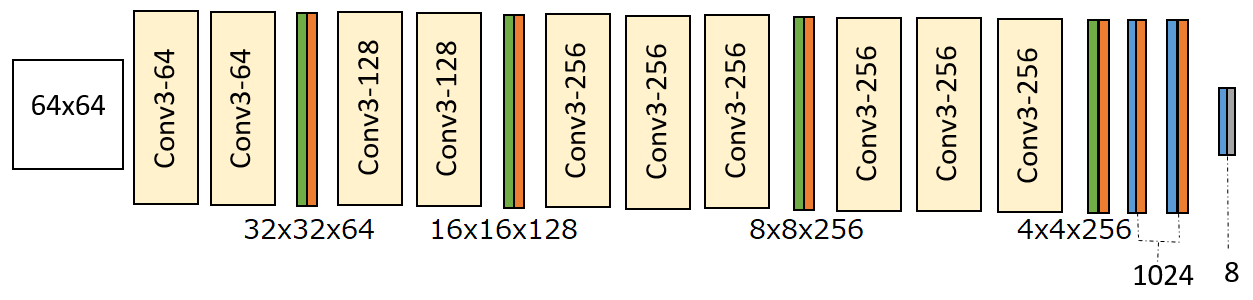
\includegraphics[width=\textwidth]{ferplus.png}
  \caption{测试使用的CNN结构}\label{fig:ferplus}
\end{figure}

整个网络结构如上图所示,输入为为$64\times 64$灰度图片,其后的黄、绿、橙、蓝、灰色分别对应于卷积层、最大池化层、Dropout层、全连接+ ReLU层、Softmax层。该网络自VGG-13修改而来,以适应低分辨率的FER数据集。
训练得到的准确率在85\% 左右,与文中得到的结果基本一致。
事实上,该准确率很大程度上是受FER+数据集自身所限。FER+数据集使用$64\times 64$的8bit灰度图片,且包含各种姿势(如侧脸、捂脸等),相比本次实验中最终需要测试的CK+、JAFFE等高分辨率正脸数据集而言,识别难度难度更大。针对前述测试数据集,下文提到的传统方法能够在更短时间、更小训练集下取得相仿甚至更高的正确率。

然而,仅仅在\cite{BarsoumICMI2016}中采用的数据集上达到这一准确率是远远不够的。我们用实验提供的训练数据进行了测试,发现由于训练数据过少,得到的模型效果并不理想,准确率较低。因此我们转而考虑采用传统的特征提取方式,在下文中将详细介绍。

\section{算法实现}

\subsection{预处理}

由于各数据集中的人脸位置并不相同,在进行表情判断前,我们先进行人脸检测。人脸检测使用传统的哈尔特征级联分类器实现,用于检测人脸所需的模型参数在各种图像处理的语言或库中均有附带,实验中我们使用MatLab内置的人脸检测模型,使用维奥拉-琼斯目标检测框架进行人脸检测。检测到人脸后将人脸切出,并统一缩放至$128\times 128$,作为后续表情识别步骤的输入。

\subsection{WLD特征提取}

WLD是Weber Local Descriptor的缩写,是近年提出的重要图像特征之一,具有很好的鲁棒性。该特征最早由\cite{chen2010wld}提出,利用了人眼视觉的生理学性质,是一种基于差分刺激和方向的特征算子。我们采用的WLD特征提取算法将图片分成$8\times 8$的小块,对每块提取WLD特征,即提取差分算子和方向算子得到二维的分布图,并将二维的分布图扩展为一维的直方图,即得到这一小块的WLD特征。由于人脸中不同位置对表情的影响是不一样的,所以对不同小块的WLD特征还要进向加权。这里我们权值的选取参照了论文\cite{wang2013feature}中的结果,如下图所示:
\begin{figure}[ht]
  \centering
  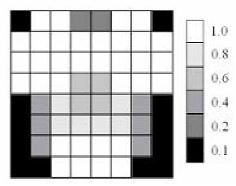
\includegraphics[width=0.5\textwidth]{WLD.jpg}
  \caption{WLD特征的权值选取}\label{fig:wldweight}
\end{figure}

\subsection{HOG特征提取}

方向梯度直方图也是图像特征提取中常用的特征。它将图像分为若干个tile,在每个tile中统计各个方向分量的分布直方图,在由若干临近的tile组成的block中对各个tile的直方图进行归一化,然后将各个tile的直方图拼接成一个向量作为该block的特征向量,最后将全图各个block的特征向量拼接起来作为全图的HOG特征。

在划分tile和block时,我们选取的参数是每个tile大小为$8\times 8$,每个block由$2\times 2$个tile组成,而相邻两个block重叠一半面积。

\subsection{最近邻判定}

在以上两种特征被提取出之后,将其拼接成一个向量,从而每张图片对应于一个特征向量。在训练时,记录下各个向量和它们相应的标签(表情)。在测试时,对输入的图片重复上述特征提取过程,得到一个特征向量。从训练的数据中找到与输入图片特征向量最近的向量,输出相应的标签作为识别结果。

注意到使用的两种特征都是统计意义下的直方图,而卡方距离常常用于衡量两个统计分布列间的差异性。因此,采用卡方距离作为衡量测试时输入图片特征向量与现有向量的距离的标准。

\section{实验结果}

\subsection{输出样例与准确率}

我们从训练集中随机均匀地选取100张图片用于测试正确率(其余留作训练数据),正确率为83\%。

以下展示判决程序运行的样例结果。这里我们将输出形式改为对单个图片进行判决,以便展示结果。如图\ref{fig:result}所示。可见,该图判决为fe(fear)类,这是一次正确的判决。
\begin{figure}[ht]
  \centering
  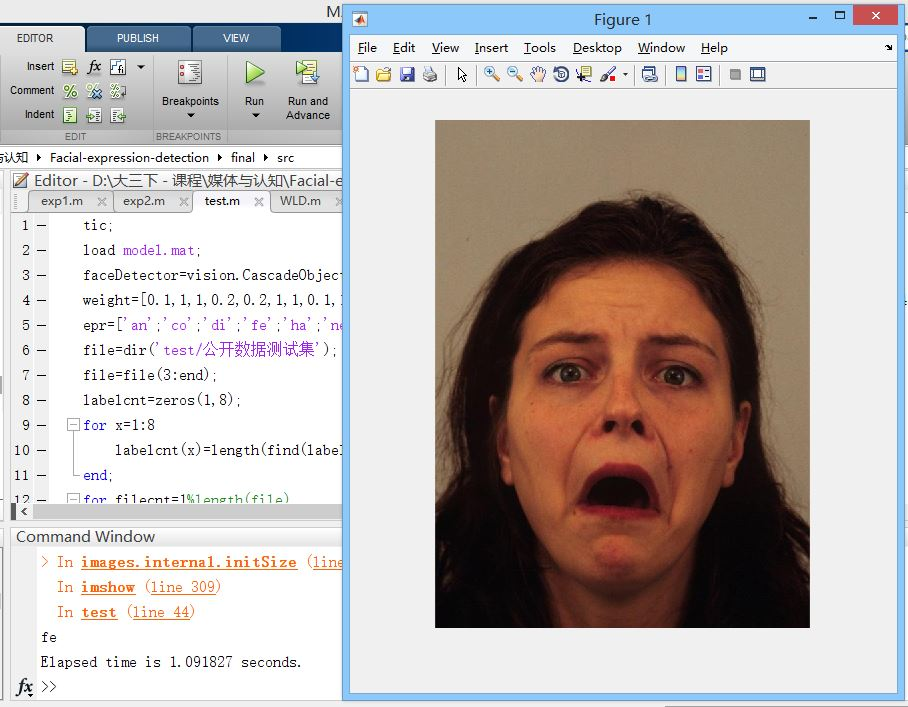
\includegraphics[width=0.8\textwidth]{result.jpg}
  \caption{一次运行的输出结果示例。}\label{fig:result}
\end{figure}

\subsection{错判样例与分析}

这里,我们选取一些错判的样例进行简要分析。这里考察的是测试数据集,由于该数据集并未提供标注,我们判断“错判”的依据是将判决的结果与人直接判决的结果进行比较。我们只是浏览了测试数据集,随机地找出一些比较典型且确定的错判样例,并进行分析。尽管这种方法带有较强的主观性,而且人直接判决的结果未必准确,但这不失为粗略评估算法的一种方法。我们希望通过观察典型的错判样例,寻找该方法的主要缺点,以及未来的改进方向。

对于图\ref{fig:error1},本判决程序将其判为happy,而人眼观察认为可能是contempt。可以发现,这幅图的人脸中两侧均上扬的嘴角和眼部与happy的图片确实有比较大的相似之处。
对于图\ref{fig:error2},本判决程序将其判为neutral,而人眼观察认为可能是sad。由于训练中大多数sad类图片并没有捂脸的动作,而且情绪体现以面部动作为主,而非眼泪,因此无法识别为sad也是可以理解的。
\begin{figure}[ht]
\begin{minipage}[t]{0.5\textwidth}
\centering
  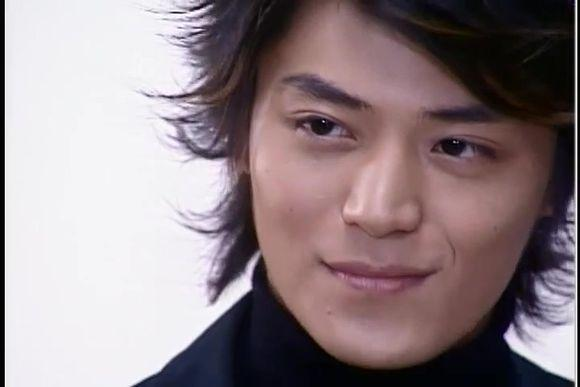
\includegraphics[width=0.8\textwidth]{0205.jpg}
  \caption{可能发生错判的图片,判决为happy,人眼观察认为可能是contempt。}\label{fig:error1}
\end{minipage}
\begin{minipage}[t]{0.5\textwidth}
\centering
  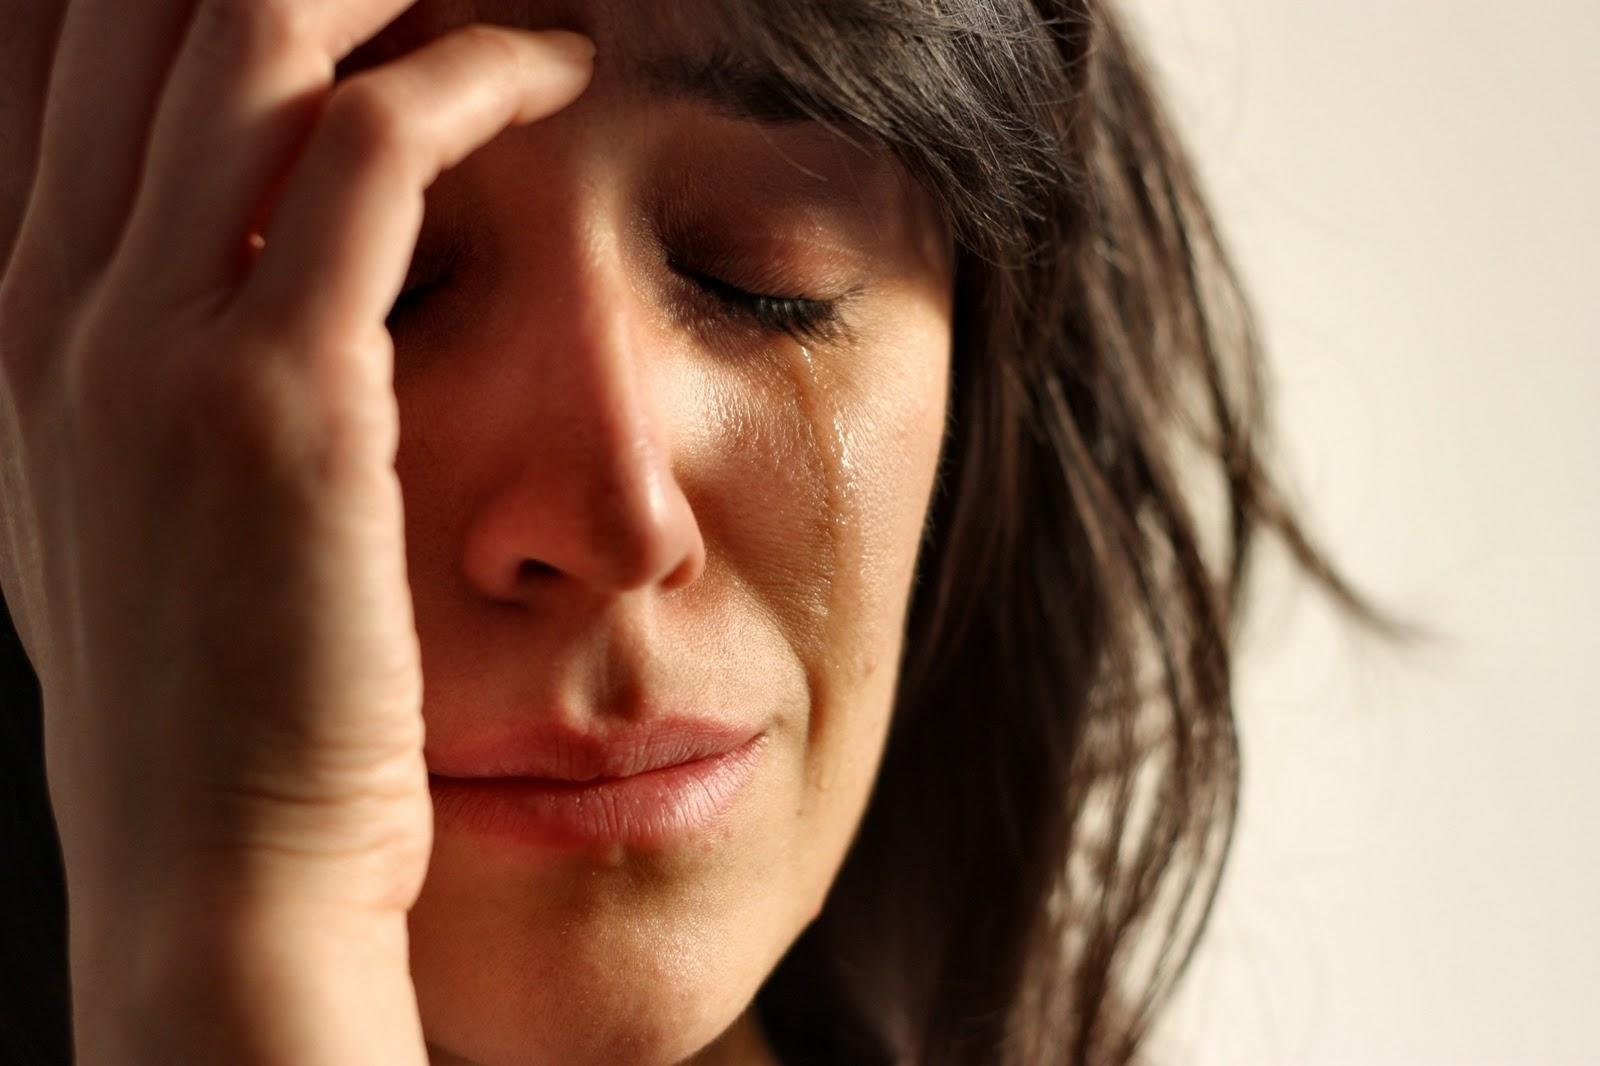
\includegraphics[width=0.8\textwidth]{0400.jpg}
  \caption{可能发生错判的图片,判决为neutral,人眼观察认为可能是sad。}\label{fig:error2}
\end{minipage}
\end{figure}

因此可见,发生的错判一方面主要来源于测试数据与训练样本间特征的不一致性,导致模型不能完全捕捉各类的特点,另一方面主要来源于一些图片自身属性就相对模糊,即使是人也较难判断,需要借助环境信息来确认。

\section{总结}

对于本实验,我们采用WLD+HOG特征提取及最近邻判别的方法完成了判决的过程。得到的准确率属于中等,还有较大的改进空间。我们目前看来,主要的改进方式包括以下几点:
\begin{itemize}
  \item 增加模型训练集的大小,用更全面、更具有代表性的样本进行训练。对于我们采用的算法,每张图片大概能得到一万维的特征向量,数据数量增加model文件会特别大,因为我们也没有选用更多的数据集,所以就没有遇到这方面的问题。但如果数据数量增大后,我的想法是,规定每个表情的图片数量(比如100张),如果图片数量过多,就采用类似Huffman树合并的思想,每个图片抽象为一个点,权重为1,然后合并距离最近的点,权重相加,新的点两合并的两点的质心(权重相当于质量),不断合并直到图片数量减小到规定的值即可。
  \item 尝试采用其他图像特征。我们曾尝试过采用LBP特征,但效果并不好,因此最后将该部分舍弃。如果未来有更加合适的图像特征提取方式被提出,可以考虑采用。
  \item 当训练样本足够大时,可以考虑重新采用神经网络训练的方法,应该可以显著提高准确率。
\end{itemize}

同时,我们感到,表情识别这项工作的难度在众多模式识别问题中是较大的,因为表情与情绪很多时候仅仅通过一幅图片很难判断,而要通过人的行为、环境等信息综合判断。从这方面看,对视频进行表情识别可能会获得更高的准确率,因为有更多的信息可以利用。

总之,经过本次实验,我们对人脸表情识别这一当前热门问题有了更加深入的了解,同时也动手实现了图像特征提取、分类、神经网络等多种机器学习的常用方法,能力得到了极大的锻炼。

最后,衷心感谢老师和助教一学期以来的付出!

\bibliographystyle{unsrt}
\bibliography{finalref}

\end{document}
